\documentclass{article}
\usepackage[utf8]{inputenc}
\usepackage{amsmath}
\usepackage{indentfirst}
\usepackage{graphicx,caption}
\usepackage[a4paper, margin=1in]{geometry}
\linespread{1.15}
\usepackage{empheq}
\usepackage[most]{tcolorbox}
\usepackage[margin=3cm]{caption}

\usepackage{xcolor,sectsty}
\definecolor{astral}{RGB}{46,116,181}
\subsectionfont{\color{astral}}
\sectionfont{\color{astral}}

\title{
\includegraphics[width=0.1\textwidth]{ufallogo.png} \\
\Huge{\color{astral}\textbf{Teoria Clássica da Radiação}}}
\author{Paulo Brandão}
\date{Maio de 2017}

\newtcbox{\mymath}[1][]{%
    nobeforeafter, math upper, tcbox raise base,
    enhanced, colframe=blue!30!black,
    colback=blue!30, boxrule=1pt,
    #1}

\begin{document}

\maketitle

\section{Introdução}

Após a unificação dos fenômenos elétricos com os fenômenos magnéticos, feita por Maxwell em torno de 1865, uma de suas consequências foi o reconhecimento de que a luz é uma onda eletromagnética que se propaga no vácuo com uma velocidade constante. Maxwell foi o primeiro a demonstrar que os campos elétricos e magnéticos satisfazem uma equação da onda e que, portanto, devem se propagar pelo espaço transmitindo energia de um ponto a outro em forma de ondas eletromagnéticas. A comprovação experimental de que era realmente possível criar um campo eletromagnético propagante no espaço, foi feita por H. Hertz no período entre 1886 e 1889. É relativamente fácil construir um aparato experimental nos dias de hoje que reproduza os mesmos efeitos que Hertz reproduziu no século 19. Todos os experimentos do tipo que Hertz construiu se baseiam em um transmissor e um receptor. O transmissor tem como objetivo produzir um movimento de cargas aceleradas gerando assim uma onda eletromagnética que será absorvida pelo receptor, alguns metros distante do transmissor. A verificação experimental da propagação das ondas eletromagnéticas por Hertz foi um passo muito importante para a validação das equações de Maxwell \footnote{A onda eletromagnética criada no laboratório por Hertz estava na faixa de frequência que hoje chamamos de microondas.}.

Em geral, o curso de eletromagnetismo começa com o estudo do campo elétrico gerado por cargas fixas no espaço com relação à um sistema de coordenadas. É demonstrado que nessa situação o vetor campo elétrico $\mathbf{E}$ não varia no tempo (porém, pode variar no espaço), e dizemos que estamos na condição de campo elétrico estático (ou eletrostática). O mesmo ocorre para campos magnéticos $\mathbf{B}$ gerados por correntes elétricas estacionárias (magnetostática). Mais adiante, estudamos algumas soluções das equações de Maxwell numa região \textit{livre} de cargas. Esse é o primeiro contato que fazemos com uma onda eletromagnética e suas propriedades de polarização, reflexão em um meio, direção de propagação, fluxo de energia, etc. Aqui, aprendemos que os campos elétricos podem variar tanto no espaço como no tempo com determinadas frequências, mas não é explicado como essas ondas eletromagnéticas são criadas em primeiro lugar. O objetivo desta aula é demonstrar como as ondas eletromagnéticas são criadas a partir de uma dada distribuição de cargas e correntes e compreender o significado de radiação.  

A discussão começa na Seção 2 com as transformações de calibre, necessárias para uma formulação mais adequada das equações de Maxwell para o tratamento da radiação. Os potenciais do campo eletromagnético serão introduzidos bem como a definição do calibre de Lorentz. Na seção 3, apresentaremos as expressões gerais para os potenciais em termos das cargas e correntes retardadas. A partir da solução geral para os potenciais, temos dois caminhos a seguir. Escolhemos discutir o campo eletromagnético gerado por uma carga carregada seguindo uma trajetória $\mathbf{w}(t)$ arbitrária, que dará origem aos potenciais de Liénard-Wiechert na seção 4. Na seção 5 calculamos os campos $\mathbf{E}$ e $\mathbf{B}$ para a carga e, finalmente, na seção 6 introduziremos o conceito de radiação eletromagnética. Alguns exemplos serão dados nas seções 7 e 8 e por fim, na seção 9, discutiremos um formalismo mais geral que dará origem à expansão em multipolos do campo eletromagnético.

\section{Transformações de Calibre}

\subsection{Potenciais do Campo Eletromagnético}

Antes de discutir o significado de radiação eletromagnética e demonstrar como ela é gerada a partir de cargas, é importante estabelecer alguns conceitos que facilitarão a análise de sistemas dinâmicos. O primeiro conceito aparece por conta da liberdade de escolha do potencial elétrico e do potencial magnético. A partir das equações de Maxwell no vácuo,
\begin{equation}
    \nabla\cdot\mathbf{E} = \frac{\rho}{\varepsilon_0}
    \label{eq11}
\end{equation}
\begin{equation}
    \nabla\cdot\mathbf{B} = 0
    \label{eq22}
\end{equation}
\begin{equation}
    \nabla\times\mathbf{E} = -\frac{\partial\mathbf{B}}{\partial t}
    \label{eq33}
\end{equation}
\begin{equation}
    \nabla\times\mathbf{B} = \mu_0\mathbf{J} + \frac{1}{c^2}\frac{\partial\mathbf{E}}{\partial t},
    \label{eq44}
\end{equation}
como $\nabla\cdot\mathbf{B}=0$, mesmo quando o campo magnético varia no tempo, é sempre possível escrever
\begin{empheq}[box=\tcbhighmath]{equation}
    \mathbf{B} = \nabla\times\mathbf{A},
    \label{eq55}
\end{empheq}
de modo que o campo magnético pode ser determinado pelo \textit{vetor potencial} $\mathbf{A}$. A situação para o campo elétrico é um pouco diferente pois $\nabla\times\mathbf{E} = -\partial\mathbf{B}/\partial t$, e não podemos escrever $\mathbf{E} = -\nabla\Phi$ por conta do termo magnético dependente do tempo. A saída é substituir a equação \eqref{eq55} na equação \eqref{eq33}:
\begin{equation}
    \nabla\times\mathbf{E} + \frac{\partial (\nabla\times\mathbf{A})}{\partial t} = \nabla\times\left( \mathbf{E} + \frac{\partial\mathbf{A}}{\partial t} \right) = 0.
\end{equation}
Assim, a generalização de $\mathbf{E} = -\nabla\Phi$ para campos dependentes do tempo é 
\begin{empheq}[box=\tcbhighmath]{equation}
    \mathbf{E} = -\frac{\partial\mathbf{A}}{\partial t} - \nabla\Phi,
    \label{eq77}
\end{empheq}
onde $\Phi$ é o \textit{potencial escalar} dependente do tempo. Resta saber se as escolhas dos potenciais das relações \eqref{eq55} e \eqref{eq77} satisfazem as equações restantes \eqref{eq11} e \eqref{eq44}. Por substituição direta é possível mostrar que as relacões
\begin{equation}
    \nabla^2 \Phi + \frac{\partial}{\partial t}(\nabla\cdot\mathbf{A}) = - \frac{\rho}{\varepsilon_0}
    \label{eq88}
\end{equation}
\begin{equation}
    \left( \nabla^2 \mathbf{A} - \frac{1}{c^2}\frac{\partial^2 \mathbf{A}}{\partial t^2}\right) - \nabla\left( \nabla\cdot\mathbf{A} + \frac{1}{c^2}\frac{\partial\Phi}{\partial t} \right) = -\mu_0\mathbf{J}
    \label{eq99}
\end{equation}
são completamente equivalentes às equações de Maxwell. Apesar da forma matemática parecer mais complicada (e é), temos uma liberdade na escolha das funções $\mathbf{A}$ e $\Phi$. Vamos supor que definimos um novo vetor potencial $\mathbf{A}'$ relacionado com o ``velho'', $\mathbf{A}$, através de
\begin{equation}
    \mathbf{A}' = \mathbf{A} + \mathbf{\alpha}
\end{equation}
onde $\mathbf{\alpha}$ é um campo vetorial. Se impormos a condição de que o novo campo magnético $\mathbf{B}'$ deve ser igual ao antigo $\mathbf{B}'$, então devemos ter
\begin{equation}
    \mathbf{B}' = \nabla\times\mathbf{A}' = \nabla\times\mathbf{A} + \nabla\times\mathbf{\alpha} = \mathbf{B} + \nabla\times\mathbf{\alpha},
\end{equation}
assim, para que $\mathbf{B}' = \mathbf{B}$, devemos garantir que $\nabla\times\mathbf{\alpha} = 0$ ou $\mathbf{\alpha} = \nabla\lambda$. Para o campo elétrico, temos
\begin{equation}
    \mathbf{E}' = -\frac{\partial\mathbf{A}'}{\partial t} -\nabla\Phi' = -\frac{\partial}{\partial t}(\mathbf{A}+\nabla\lambda) - \nabla\Phi'
\end{equation}
e, para o mesmo permanecer inalterado, $\mathbf{E} = \mathbf{E}'$, devemos ter $\nabla\Phi = \nabla(\Phi' +\partial\lambda/\partial t)$ ou, equivalentemente,
\begin{equation}
    \Phi' = \Phi - \frac{\partial\lambda}{\partial t}.
\end{equation}
Concluímos que as mudanças de $(\mathbf{A},\Phi)$ para $(\mathbf{A}',\Phi')$ dadas por
\begin{equation}
    \mathbf{A}' = \mathbf{A} + \nabla\lambda
\end{equation}
\begin{equation}
    \Phi' = \Phi - \frac{\partial\lambda}{\partial t}
\end{equation}
não afetam os valores dos campos $\mathbf{E}$ e $\mathbf{B}$. As mudanças no vetor potencial e no potencial escalar são chamadas de \textbf{transformações de calibre} e iremos explorar a liberdade na escolha da função $\lambda$ para simplificar os cálculos que seguem.

\subsection{O Calibre de Lorentz}

A ideia é escolher uma função $\lambda$ tal que 
\begin{equation}
    \nabla\cdot\mathbf{A} + \frac{1}{c^2}\frac{\partial\Phi}{\partial t} = 0.
    \label{lorentz}
\end{equation}
Essa escolha da função $\lambda$ que satisfaz a relação acima é chamada de \textbf{Calibre de Lorentz}. Surge a importante pergunta: Será que é possível fazer isso? A resposta é: sim. Porém não iremos demonstrá-la aqui por ser apenas um exercício de cálculo sem muitas vantagens do ponto de vista físico. O aluno que quiser se aprofundar mais nesse ponto, pode consultar as referências listadas no plano de aula. Utilizando a relação \eqref{lorentz} nas equações \eqref{eq88} e \eqref{eq99}, obtemos as duas relações completamente equivalentes às equações de Maxwell
\begin{empheq}[box=\tcbhighmath]{equation}
    \nabla^2 \mathbf{A} - \frac{1}{c^2}\frac{\partial^2 \mathbf{A}}{\partial t^2} = -\mu_0 \mathbf{J}
    \label{eq1818}
\end{empheq}
\begin{empheq}[box=\tcbhighmath]{equation}
    \nabla^2 \Phi - \frac{1}{c^2}\frac{\partial^2 \Phi}{\partial t^2} = -\frac{1}{\varepsilon_0} \rho.
    \label{eq1919}
\end{empheq}
Ambas as equações possuem a mesma forma matemática. Os matemáticos chamam as relações acima de equações diferenciais parciais não-homogêneas, pois contém um termo de fonte no lado direito da equação. Nosso próximo objetivo é encontrar a solução dessas equações. Observe também que os potenciais se desacoplaram, isto é, a equação para o vetor potencial $\mathbf{A}$ não depende de uma maneira direta dos valores do potencial escalar $\Phi$ e vice-versa. Assim, através da escolha do Calibre de Lorentz, conseguimos simplificar as relações mais complicadas \eqref{eq88} e \eqref{eq99}.

Existe um outro tipo de calibre que é geralmente utilizado em outros contextos e que mostrou-se ser muito útil. O \textbf{Calibre de Coulomb} aparece quando escolhemos uma função $\lambda$ tal que $\nabla\cdot\mathbf{A} = 0$. A vantagem desse calibre é que a equação resultante para o potencial $\Phi$ pode ser facilmente resolvida. A desvantagem é que a equação para $\mathbf{A}$ se torna bastante complicada. Por conta disso, não iremos utilizar o calibre de Coulomb nessa aula. 


\section{Potenciais Retardados}

No estudo da eletrostática, vimos que para uma distribuição estacionária de cargas $\rho(\mathbf{r})$, o potencial elétrico satisfaz a equação diferencial parcial não-homogênea $\nabla^2 \Phi = -\rho/\varepsilon_0$ cuja solução vale
\begin{equation}
    \Phi(\mathbf{r}) = \frac{1}{4\pi\varepsilon_0}\int_{V}\frac{\rho(\mathbf{r}')}{|\mathbf{r} - \mathbf{r}'|}dv',
    \label{eq1}
\end{equation}
onde $V$ é o volume da distribuição de cargas, $\mathbf{r}$ é o vetor posição do campo e $\mathbf{r}'$ o vetor posição na distribuição de cargas $\rho$. Da mesma forma, para uma corrente $\mathbf{J}(\mathbf{r}')$ estacionária, o vetor potencial satisfaz a equação diferencial parcial não-homogênea $\nabla^2 \mathbf{A} =  -\mu_0 \mathbf{J}$ cuja solução é dada por 
\begin{equation}
    \mathbf{A}(\mathbf{r}) = \frac{\mu_{0}}{4\pi}\int_{V}\frac{\mathbf{J}(\mathbf{r}')}{|\mathbf{r} - \mathbf{r}'|}dv'.
    \label{eq2}    
\end{equation}
Conhecendo a distribuição espacial do potencial elétrico e do vetor potencial, os campos $\mathbf{E}(\mathbf{r})$ e $\mathbf{B}(\mathbf{r})$ são calculados através das relações $\mathbf{E} = -\nabla\Phi$ e $\mathbf{B} = \nabla\times\mathbf{A}$. No caso mais geral, onde as cargas e correntes variam com o tempo, as relaçoes \eqref{eq1} e \eqref{eq2} não podem ser utilizadas. O próximo objetivo desta aula será generalizar as relações acima para distribuições de carga e corrente que dependem do tempo $t$. Em outras palavras, iremos encontrar as soluções das equações \eqref{eq1818} e \eqref{eq1919}.

Existem basicamente duas formas de se obter as equações mais gerais para $\Phi(\mathbf{r},t)$ e $\mathbf{A}(\mathbf{r},t)$, soluções das equações \eqref{eq1818} e \eqref{eq1919}. A primeira maneira tem um caráter mais físico e intuitivo e envolve apenas o conhecimento de que o campo eletromagnético é transmitido com uma velocidade finita. O segundo envolve a força bruta da matemática e exige o conhecimento de como resolver equações diferenciais não-homogêneas. Como o primeiro método fornece o mesmo resultado do segundo, irei seguir o caminho mais físico e intuitivo \footnote{O resultado a ser obtido pelo método intuitivo é idêntico ao método mais técnico de solução de equações diferenciais não-homogêneas, porém esse último depende do tipo de Calibre utilizado. As equações são idênticas no Calibre de Lorentz.}. O aluno que desejar verificar os resultados obtidos de uma forma mais técnica deve trabalhar no problema 1 da lista de exercícios. Acontece que a única mudança a ser feita nas Equações \eqref{eq1} e \eqref{eq2} para o caso onde $\rho = \rho(\mathbf{r},t)$ e $\mathbf{J} = \mathbf{J}(\mathbf{r},t)$ é a substituição do tempo $t$, que aparece \textit{dentro do integrando}, pelo \textbf{tempo retardado}:
\begin{equation}
t_r = t - \frac{|\mathbf{r} - \mathbf{r}'|}{c},
\label{eq3}
\end{equation}
onde $c$ é a velocidade da luz no vácuo. Dessa forma, as equações \eqref{eq1} e \eqref{eq2} podem ser generalizadas para
\begin{empheq}[box=\tcbhighmath]{equation}
    \Phi(\mathbf{r},t) = \frac{1}{4\pi\varepsilon_0}\int_{V}\frac{\rho(\mathbf{r}',t_r)}{|\mathbf{r} - \mathbf{r}'|}dv' = \frac{1}{4\pi\varepsilon_0}\int_{V} \rho\left(\mathbf{r}',t - \frac{|\mathbf{r} - \mathbf{r}'|}{c}\right) \frac{dv'}{|\mathbf{r} - \mathbf{r}'|}, 
    \label{eq4}    
\end{empheq}
\begin{empheq}[box=\tcbhighmath]{equation}
    \mathbf{A}(\mathbf{r},t) = \frac{\mu_{0}}{4\pi}\int_{V}\frac{\mathbf{J}(\mathbf{r}',t_r)}{|\mathbf{r} - \mathbf{r}'|}dv' = \frac{\mu_{0}}{4\pi}\int_{V}\mathbf{J}\left(\mathbf{r}',t - \frac{|\mathbf{r} - \mathbf{r}'|}{c}\right)\frac{dv'}{|\mathbf{r} - \mathbf{r}'|}.
    \label{eq5}    
\end{empheq}
No Calibre de Lorentz, os campos elétrico e magnético são dados agora por $\mathbf{E} = -\nabla\Phi - \partial \mathbf{A}/\partial t$ e $\mathbf{B} = \nabla\times\mathbf{A}$. Para compreender fisicamente o papel do tempo retardado $t_r$, considere uma distribuição de cargas e correntes localizadas, isto é, que ocupam uma região finita do espaço, como ilustra a Figura 1. A distância da origem do sistema de coordenadas $O$ até um ponto da fonte é $|\mathbf{r}'|$ enquanto que a distância desse ponto da fonte até o ponto de observação $P$ vale $|\mathbf{r}-\mathbf{r}'|$. Essa distância, do ponto na fonte $\mathbf{r}'$ até o ponto de observação $\mathbf{r}$, será percorrida pelo campo eletromagnético num tempo $|\mathbf{r}-\mathbf{r}'|/c$. Dessa forma, o sinal emitido pelo ponto $\mathbf{r}'$ acontecerá no tempo $t_r$ enquanto que o sinal recebido no ponto $P$ acontecerá no tempo $t$, onde $t_r$ e $t$ estão relacionados pela Equação \eqref{eq3}. Esse é, portanto, o significado da estranha dependência temporal dos termos no integrando das relações \eqref{eq4} e \eqref{eq5}. O mesmo resultado é obtido através de uma análise laboriosa partindo das equações de Maxwell não-homogêneas. O estudante demonstrará, através dos problemas da lista de exercício, que \eqref{eq4} e \eqref{eq5} são de fato as soluções para o nosso problema.

\begin{figure}[ht]
\centering
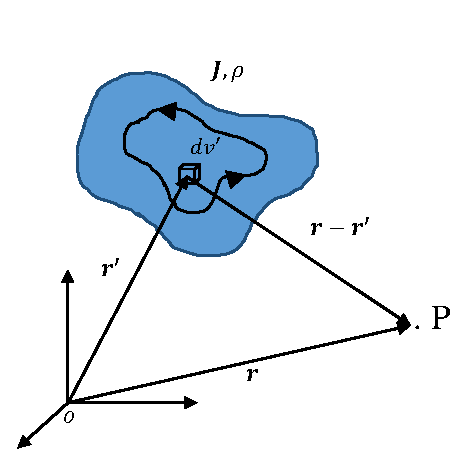
\includegraphics[width=7cm]{fig1.pdf}
\caption{Geometria do problema. Uma fonte, consistindo de cargas $\rho$ e correntes $\mathbf{J}$ que variam no tempo, criam um campo eletromagnético no ponto $P$.}
\end{figure}

É fácil perceber que as integrais \eqref{eq4} e \eqref{eq5} são extremamente complicadas de se resolver até para as distribuições de cargas mais simples. Na próxima seção iremos estudar o caso particular onde apenas uma carga $q$ move-se no espaço descrevendo uma \textit{dada} trajetória $\mathbf{r}(t)$. Com isso, mostraremos que existem dois tipos de campos associados ao movimento da carga, um deles sobrevive à grandes distâncias da fonte e o outro não. A parte do campo que sobrevive para $|\mathbf{r}|\rightarrow\infty$ será chamada de \textbf{radiação}.

Caso o problema fosse formulado em termos do Calibre de Coulomb, pode ser demonstrado que a solução para o potencial $\Phi$ seria da forma
\begin{equation}
    \Phi(\mathbf{r},t) = \frac{1}{4\pi\varepsilon_0}\int_{V}\frac{\rho(\mathbf{r}',t)}{|\mathbf{r} - \mathbf{r}'|}dv',
\end{equation}
isto é, sem o tempo retardado. Pode parecer que a causalidade, tão importante na física, estaria sendo violada. No entanto, o vetor potencial $\mathbf{A}$ carrega, neste caso, toda a informação causal. Lembre-se de que o sinal físico é carregado \textit{pelos campos} e não pelos potenciais, de forma que o Calibre de Coulomb também não viola os conceitos relativísticos.

Nesse ponto, o curso pode se dividir em duas partes. Na primeira parte, estudamos os campos gerados por uma partícula carregada que percorre uma \textit{dada} trajetória arbitrária $\mathbf{w}(t)$ no espaço. Na segunda parte, é considerado o caso geral onde a densidade de carga do objeto depende periodicamente do tempo. Isto é, para um ponto fixo no espaço, a densidade de carga deve ser uma função periódica do tempo. O segundo percurso dará origem à expansão em multipolos do campo eletromagnético e representa um dos grandes avanços da teoria de radiação clássica com inúmeras aplicações em sistemas físicos. Por outro lado, um tratamento sistemático da expansão em multipolos requer uma matemática relativamente avançada e, como estamos em um nível de graduação, escolhi discutir apenas a radiação gerada por cargas pontuais. No final da aula discutirei um pouco as ideias envolvidas na expansão em multipolos bem como indicarei possíveis referências para que o estudante mais interessado possa iniciar um estudo mais aprofundado.

\section{Os Potenciais de Liénard-Wiechert}

Vamos aplicar as relações obtidas na seção anterior num problema particularmente simples de ser formulado: dada a trajetória $\mathbf{w}(t)$ de uma partícula carregada, calcule os potenciais $\Phi$ e $\mathbf{A}$ para qualquer posição $\mathbf{r}$ e tempo $t$. Podemos escrever a densidade de carga $\rho$ como
\begin{equation}
    \rho(\mathbf{r},t) = q\delta[\mathbf{r}-\mathbf{w}(t)].
    \label{eq25}
\end{equation}
Após substituir a densidade \eqref{eq25} na equação \eqref{eq4} para o potencial escalar $\Phi(\mathbf{r},t)$, ficamos com a integral
\begin{equation}
    \Phi(\mathbf{r},t) = \frac{q}{4\pi\varepsilon_0}\int_{V} \delta\left[ \mathbf{r}' - \mathbf{w}\left(t-\frac{|\mathbf{r} - \mathbf{r}'|}{c}\right) \right] \frac{dv'}{|\mathbf{r} - \mathbf{r}'|}
    \label{eq26}
\end{equation}
que, infelizmente, não é facilmente calculada. É útil dar um passo para trás e reescrever a integral \eqref{eq26} na forma
\begin{equation}
    \Phi(\mathbf{r},t) = \frac{q}{4\pi\varepsilon_0}\int_{V}dv'\int dt' \delta\left[ \mathbf{r}' - \mathbf{w}\left(t'\right) \right]\delta\left( t'- t + \frac{|\mathbf{r}-\mathbf{r}'|}{c} \right) \frac{1}{|\mathbf{r} - \mathbf{r}'|}.   
\end{equation}
Podemos agora resolver a integral em $dv'$ facilmente:
\begin{equation}
    \Phi(\mathbf{r},t) = \frac{q}{4\pi\varepsilon_0}\int dt' \delta\left( t'- t + \frac{|\mathbf{r}-\mathbf{w}(t')|}{c} \right) \frac{1}{|\mathbf{r} - \mathbf{w}(t')|}.   
\end{equation}
Para o próximo passo, defina uma nova variável $u$ dada por
\begin{equation}
    u = t'- t + \frac{|\mathbf{r}-\mathbf{w}(t')|}{c} = t' - t + \frac{\sqrt{(x-w_x (t'))^2 + (y-w_y (t'))^2 + (z-w_z (t'))^2}}{c}
\end{equation}
\begin{equation}
    \frac{du}{dt'} = 1 - \frac{[(x-w_x(t'))\dot{w}_x(t')^2 + (y-w_y(t'))\dot{w}_y(t')^2 + (z-w_z(t'))\dot{w}_z(t')^2 ]}{c\sqrt{(x-w_x (t'))^2 + (y-w_y (t'))^2 + (z-w_z (t'))^2}} = 1 - \hat{\mathbf{n}}(t')\cdot\frac{\mathbf{v}(t')}{c},
\end{equation}
onde
\begin{equation}
    \hat{\mathbf{R}}(t') = \frac{\mathbf{r} - \mathbf{w}(t')}{|\mathbf{r} - \mathbf{w}(t')|}
\end{equation}
e
\begin{equation}
    \mathbf{v}(t') = \frac{d\mathbf{w}(t')}{dt'}.
\end{equation}
Podemos reescrever a integral agora em termos da nova variável $u$ e integrar diretamente:
\begin{equation}
\begin{split}
    \Phi(\mathbf{r},t) &= \frac{q}{4\pi\varepsilon_0}\int du \frac{1}{|\mathbf{r} - \mathbf{w}(t'(u))|}\cdot\frac{1}{1 - \hat{\mathbf{R}}(t'(u))\cdot\frac{\mathbf{v}(t'(u))}{c}}\delta(u)\\
                       &= \frac{q/4\pi\varepsilon_0}{|\mathbf{r} - \mathbf{w}(t'(0))|[1 - \hat{\mathbf{R}}(t'(0))\cdot\frac{\mathbf{v}(t'(0))}{c}]}\\
                       &= \frac{q/4\pi\varepsilon_0}{|\mathbf{r} - \mathbf{w}(t_r)|\left[1 - \hat{\mathbf{R}}(t_r)\cdot\frac{\mathbf{v}(t_r)}{c}\right]}\bigg\rvert_{t_r=t-|\mathbf{r}-\mathbf{w}(t_r)|/c}.
\end{split}
\end{equation}
Fica como exercício para o aluno (ver lista de exercícios) demonstrar a expressão para o potencial vetor $\mathbf{A}$. Em resumo, os potenciais dados por:
\begin{empheq}[box=\tcbhighmath]{equation}
\Phi(\mathbf{r},t) = \frac{q/4\pi\varepsilon_0}{|\mathbf{r} - \mathbf{w}(t')|\left[1 - \hat{\mathbf{R}}(t')\cdot\frac{\mathbf{v}(t')}{c}\right]}\bigg\rvert_{t'=t-|\mathbf{r}-\mathbf{w}(t')|/c}
\label{eq34}
\end{empheq}
e
\begin{empheq}[box=\tcbhighmath]{equation}
    \mathbf{A}(\mathbf{r},t) = \frac{\mu_0}{4\pi}\frac{\mathbf{v}(t')}{|\mathbf{r} - \mathbf{w}(t')|\left[1 - \hat{\mathbf{R}}(t')\cdot\frac{\mathbf{v}(t')}{c}\right]}\bigg\rvert_{t'=t-|\mathbf{r}-\mathbf{w}(t')|/c}
    \label{eq35}
\end{empheq}
são conhecidos como \textbf{Potenciais de Liénard-Wiechert}. Perceba a estrutura das equações acima. Primeiramente, é necessário conhecer o tempo retardado $t'$ em função de $(\mathbf{r},t)$ para depois substituir nas equações dos potenciais. Dependendo do formato da trajetória da carga, esse primeiro passo pode ser bastante complicado. Nosso próximo objetivo é calcular os campos elétrico e magnético e, finalmente, definir o que queremos dizer com radiação de um campo eletromagnético. 
\begin{figure}[ht]
\centering
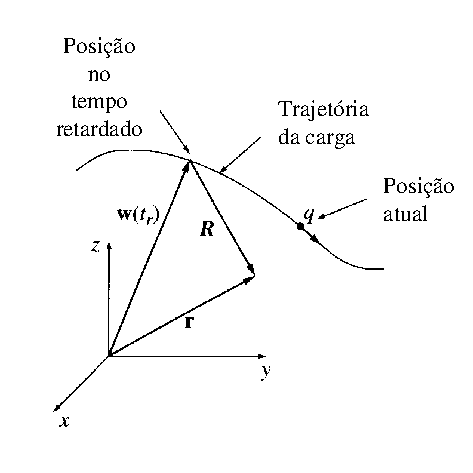
\includegraphics[width=6cm]{fig2.pdf}
\caption{Geometria de uma carga pontual se movendo numa trajetória $\mathbf{r}_e (t')$.}
\end{figure}


\section{Os Campos de Liénard-Wiechert}

De posse dos potenciais \eqref{eq34} e \eqref{eq35}, podemos calcular os campos $\mathbf{E}$ e $\mathbf{B}$ diretamente utilizando as equações \eqref{eq55} e \eqref{eq77}. O problema em tomar derivadas diretamente nas equações \eqref{eq34} e \eqref{eq35} é que as derivadas serão em termos de $t$ e $\mathbf{r}$ enquanto que a expressão dos potenciais está escrita em termos de $t_r$ que, por sua vez, é função tanto de $t$ como de $\mathbf{r}$ através da relação implícita
\begin{equation}
    c(t_r - t) = |\mathbf{r}-\mathbf{w}(t_r)|.
\end{equation}
Para piorar, escrever $t'$ em termos de $(\mathbf{r},t)$ vai depender de cada tipo de trajetória. É possível, entretanto, escrever uma equação final para os campos. O preço que pagamos para obter essas expressões é a quantidade imensa de cálculos que devem ser feitos para obtê-las. Assim, apenas mostrarei os resultados e o estudante poderá trabalhar por ele mesmo resolvendo a lista de exercícios. Os campos são dados por

\begin{empheq}[box=\tcbhighmath]{equation}
\mathbf{E}(\mathbf{r},t) = \frac{q}{4\pi\varepsilon_0}\left[ \frac{(\hat{\mathbf{R}}-\mathbf{v}/c)(1-v^2/c^2)}{(1-\hat{\mathbf{R}}\cdot\mathbf{v}/c)^3 R^2} + \frac{\hat{\mathbf{R}}\times[(\hat{\mathbf{R}}-\mathbf{v}/c)\times\mathbf{a}/c]}{c(1-\hat{\mathbf{R}}\cdot\mathbf{v}/c)^3 R} \right]\bigg\rvert_{t_r}
\label{eq37}
\end{empheq}
e
\begin{empheq}[box=\tcbhighmath]{equation}
\mathbf{B}(\mathbf{r},t) = \frac{\hat{\mathbf{R}} \times \mathbf{E}}{c}\bigg\rvert_{t_r},
\label{eq38}
\end{empheq}
onde $\mathbf{a} = \dot{\mathbf{v}}$ é a aceleração da partícula. Vários aspectos importantes podem ser percebidos através de uma inspeção das equações \eqref{eq37} e \eqref{eq38}. Primeiramente, note que se a carga não estiver em movimento, $\mathbf{v} = 0$, o campo elétrico é dado por
\begin{equation}
    \mathbf{E}_{v=0} = \frac{q\hat{\mathbf{R}}}{4\pi\varepsilon_0 R^2},
\end{equation}
como esperado. Vale enfatizar o aparecimento de fatores do tipo $1-v^2 /c^2$ e $1-\hat{\mathbf{R}}\cdot\mathbf{v}/c$ que estão diretamente ligados à teoria da relatividade de Albert Einstein, como iremos ver mais adiante no curso. Observe também que o campo magnético é sempre perpendicular ao campo elétrico. A direção na qual a partícula se move também desempenha um papel muito importante com relação ao ponto onde estamos observando os campos, como pode ser visto pela existência de produtos vetoriais e escalaras na equação. Por último, note que os dois termos da equação \eqref{eq37} diferem principalmente pela sua dependência em $R$. O primeiro termo se comporta como $\sim 1/R^2$ enquanto que o segundo se comporta como $\sim 1/R$. Mostraremos na próxima seção que o segundo termo é o responsável pela radiação emitida pela partícula carregada. Mas primeiro precisamos definir mais precisamente o que significa radiação eletromagnética.

\section{O Que é Radiação?}

Radiação é o fluxo de energia transmitido através do campo eletromagnético que se propaga irreversivelmente de uma fonte ``para o infinito''. Para que uma carga emita radiação é necessário que ela esteja \textit{acelerada}. Como podemos calcular o fluxo de energia eletromagnética à uma distância muito grande de uma distribuição de cargas localizadas? A taxa de transferência de energia por unidade de tempo e área é dada pelo vetor de Poynting $\mathbf{S}$. Assim, a energia por unidade de tempo, $P$ que passa por uma superfície é calculada por
\begin{equation}
    P(r) = \oint \mathbf{S}\cdot d\mathbf{a} = \frac{1}{\mu_0}\oint (\mathbf{E}\times\mathbf{B})\cdot d\mathbf{a}.
\end{equation}
A energia irradiada (isto é, a energia em forma de radiação) é o limite dessa quantidade quando $r\rightarrow\infty$:
\begin{equation}
    P_{\text{rad}} = \lim_{r\rightarrow\infty}P(r).
\end{equation}
A quantidade $P_{\text{rad}}$ representa a energia por unidade de tempo que é irradiada para o infinito e nunca volta. Como deve se comportar o campo para que $P_{\text{rad}} \neq 0$? O integrando é composto pelo ``produto'' de dois campos e multiplicados pelo elemento de área $da \sim R^2$. Se, por exemplo, os campos possuem a dependência $\mathbf{E}\sim 1/r^2$ e $\mathbf{B}\sim 1/r^2$ então 
\begin{equation}
    \mathbf{E}\times\mathbf{B}\cdot d\mathbf{a} \sim \frac{1}{r^2}\frac{1}{r^2}r^2 \sim \frac{1}{r^2}
\end{equation}
que vai a zero quando $r\rightarrow\infty$, e, portanto, $P_{\text{rad}} = 0$. Assim, para que as fontes irradiem, é necessária uma dependência de, pelo menos, $1/r$ em cada termo de campo.

Observe agora a dependência em $R$ nos campos descritos pelas relações \eqref{eq37} e \eqref{eq38}, derivadas na seção anterior. Fica fácil perceber que o segundo termo da equação \eqref{eq37} é o responsável pela radiação emitida pela partícula carregada que descreve a trajetória $\mathbf{w}(t)$. Vamos nomear o segundo termo de $\mathbf{E}_{\text{rad}}$:
\begin{empheq}[box=\tcbhighmath]{equation}
    \mathbf{E}_{\text{rad}}(\mathbf{r},t) = \frac{q}{4\pi\varepsilon_0} \frac{\hat{\mathbf{R}}\times[(\hat{\mathbf{R}}-\mathbf{v}/c)\times\mathbf{a}/c]}{c(1-\hat{\mathbf{R}}\cdot\mathbf{v}/c)^3 R} \bigg\rvert_{t_r}.
    \label{eq43}
\end{empheq}
É fácil perceber também que ele depende exclusivamente da aceleração da partícula: Se $\mathbf{a} = \dot{\mathbf{v}} = 0$ então $\mathbf{E}_{\text{rad}} = 0$. Demonstramos então explicitamente o fato de que para uma carga irradiar, ela precisa estar acelerada.

\section{Radiação de uma Carga Acelerada com Velocidade Baixa}

Podemos utilizar a equação da potência irradiada $P(r)$ para o caso particular onde a carga percorre uma trajetória $\mathbf{w}(t)$. Se a velocidade da partícula carregada for muito menor que a velocidade da luz $c$ (partícula não-relativística), a expressão \eqref{eq43} simplifica para
\begin{equation}
    \mathbf{E}_{\text{rad}}(\mathbf{r},t) \approx \frac{q}{4\pi\varepsilon_0 c^2}\frac{\hat{\mathbf{R}}\times(\hat{\mathbf{R}}\times\mathbf{a})}{R} = \frac{q}{4\pi\varepsilon_0 c^2} \frac{[(\hat{\mathbf{R}}\cdot\mathbf{a})\hat{\mathbf{R}} - \mathbf{a}]}{R} ,
    \label{eq444}
\end{equation}
e, para o campo magnético, podemos escrever
\begin{equation}
    \mathbf{B}_{\text{rad}}(\mathbf{r},t) = \frac{\hat{\mathbf{R}} \times \mathbf{E}_{\text{rad}}}{c} = -\frac{q}{4\pi\varepsilon_0 c^3}\frac{\hat{\mathbf{R}}\times\mathbf{a}}{R}
    \label{eq455}
\end{equation}
e, como é equivalente tomar o limite $c\rightarrow\infty$, podemos assumir que $t \approx t_r$, de modo que os termos das expressões \eqref{eq444} e \eqref{eq455} podem ser escritos no tempo real $t$ e \textbf{não} no tempo retardado $t_r$. Observe que o campo elétrico está polarizado no plano formado pelos vetores $\hat{\mathbf{E}}$ e $\mathbf{a}$ enquanto que o campo magnético é sempre perpendicular ao campo elétrico (verifique isso calculando $\mathbf{E}_{\text{rad}}\cdot\mathbf{B}_{\text{rad}}$ diretamente).

Vamos considerar agora a potência irradiada pela partícula. Primeiro devemos calcular o fluxo de energia através do vetor de Poynting:
\begin{equation}
\begin{split}
    \mathbf{S} &= \frac{1}{\mu_0}\mathbf{E}_{\text{rad}}\times\mathbf{B}_{\text{rad}}\\
               &= \frac{1}{\mu_0 c}[(\mathbf{E}_{\text{rad}}\cdot\mathbf{E}_{\text{rad}})\hat{\mathbf{R}} - (\mathbf{E}_{\text{rad}}\cdot\hat{\mathbf{R}})\mathbf{E}_{\text{rad}}]\\
               &= \frac{E_{\text{rad}}^{2}}{\mu_0 c}\hat{\mathbf{R}}\\
               &= \frac{q^2 a^2 \sin^2\theta}{16\pi^2 c^3 \varepsilon_0 R^2}\hat{\mathbf{R}},
\end{split}
\end{equation}
onde $\theta$ é o ângulo entre $\mathbf{a}$ e $\hat{\mathbf{R}}$. A radiação emitida por ângulo sólido pode ser calculada pela projeção do fluxo de energia na área $d\mathbf{A} = R^2 d\Omega \hat{\mathbf{R}}$:
\begin{equation}
dP = \mathbf{S}\cdot d\mathbf{A} = \mathbf{S}\cdot\hat{\mathbf{R}} R^2 d\Omega
\end{equation}
\begin{empheq}[box=\tcbhighmath]{equation}
    \frac{dP}{d\Omega} = R^2 \mathbf{S}\cdot\hat{\mathbf{R}} = \frac{E_{\text{rad}}^{2}}{\mu_0 c}
               = \frac{q^2 a^2 \sin^2\theta}{16\pi^2 c^3 \varepsilon_0} 
\end{empheq}
Observe que a direção da radiação emitida depende apenas da aceleração e não, explicitamente, da velocidade $\mathbf{v}$. A figura 3 ilustra a direção da radiação emitida em duas situações. Na parte (a) da figura, a trajetória da partícula é acelerada mas numa reta. A direção máxima de emissão de radiação é sempre perpendicular ao vetor aceleração. Na parte (b) da mesma figura, a partícula percorre uma trajetória circular e é fácil de perceber que a direção da radiação emitida nesse caso está na direção da velocidade, sempre perpendicular à aceleração. Esse segundo caso se parece com os faróis acesos de um carro quando o mesmo faz uma curva, iluminando o que está diretamente a frente.

Podemos utilizar a equação para a radiação emitida por ângulo sólido para calcular a potência total emitida pela carga que atravessa uma esfera de raio infinito:
\begin{equation}
    P = \int \frac{dP}{d\Omega}d\Omega = \frac{q^2 a^2}{16\pi^2 c^3 \varepsilon_0} \int \sin^2\theta d\Omega = \frac{q^2 a^2}{16\pi^2 c^3 \varepsilon_0} \frac{8\pi}{3}
\end{equation}
\begin{empheq}[box=\tcbhighmath]{equation}
P = \frac{q^2 a^2}{6 \pi c^3 \varepsilon_0}
\end{empheq}
que é a famosa \textbf{fórmula de Larmor} para a potência irradiada por uma partícula que se move com uma velocidade muito pequena comparada à velocidade da luz e com aceleração $a$.

\begin{figure}[ht]
\centering
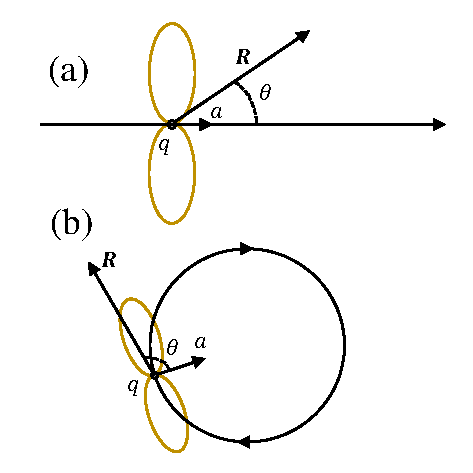
\includegraphics[width=6cm]{fig3.pdf}
\caption{Radiação emitida por uma carga pontual $q$ que se move numa trajetória (a) linear e (b) circular. }
\end{figure}

Fica claro a partir desses dois casos particulares que a situação mais geral, onde a partícula se movimenta com uma velocidade próxima da velocidade da luz, pode ser bastante complicado. A grande parte da complicação vem do fato de que a taxa de energia eletromagnética emitida pela partícula depende da posição escolhida. Isto é, a taxa na qual a energia é recebida através de uma esfera de raio infinito é diferente da taxa de energia emitida pela partícula na posição da mesma. Uma analogia mecânica pode ajudar a esclarecer esse fenômeno, Imagine que uma arma atira balas de um carro em direção à um alvo fixo no asfalto. Se o carro estiver se movendo na direção do alvo, a taxa de saída de balas do revólver é menor que a taxa de impacto das balas no alvo, em virtude do movimento relativo entre o carro e o asfalto. A expressão para a potência total emitida por uma partícula relativística é dada por
\begin{equation}
    P_{\text{rel}} = \frac{\mu_0 q^2 \gamma^6}{6 \pi c}\left( a^2 - \left| \frac{\mathbf{v}\times\mathbf{a}}{c} \right|^2 \right),
    \label{eq51}
\end{equation}
onde $\gamma = 1/\sqrt{1-v^2 / c^2}$. O fator $\gamma^6$ indica que que a potência aumenta muito quando a velocidade da carga se aproxima da velocidade da luz. É importante enfatizar que a equação \eqref{eq51} representa a taxa de perda de energia vista por um observador posicionado na posição instantânea da partícula. Essa quantidade \textit{não} é a mesma que a perda de energia vista por um observador localizado longe da carga, que mais complicada devido ao efeito de retardação da radiação, como foi discutido anteriormente. A distribuição da radiação emitida é bem mais complicada e podemos separar em dois casos particulares. No primeiro caso, a aceleração e a velocidade possuem a mesma direção


\section{Discussão Final e Conclusões}

Discutimos nessa aula um caso particular de radiação eletromagnética gerada por uma carga que percorre uma trajetória pré-determinada $\mathbf{w}(t)$. No entanto, é fácil observar que esse método consiste numa aproximação que não é realizada em prática. Isso se deve ao fato de que a carga perde energia durante seu movimento e, portanto, não é esperado que ela permaneça na mesma trajetória para sempre (se nenhuma outra força atua na carga, claro). Além disso, o próprio campo pode influenciar o movimento da carga. Tal efeito é chamado de \textit{reação de radiação} e não foi discutido aqui. Um outro ponto importante que não foi tocado nessa aula é a radiação gerada por uma configuração de cargas periódica no tempo. Isto é, olhando para as equações \eqref{eq4} e \eqref{eq5}, podemos desenvolver uma teoria geral onde a densidade de carga $\rho$ e a densidade de corrente $\mathbf{J}$ são escritas na forma $\rho(\mathbf{r},t) = \rho(\mathbf{r})e^{-i\omega t}$ e $\mathbf{J}(\mathbf{r},t) = \mathbf{J}(\mathbf{r})e^{-i\omega t}$, onde $\omega$ representa a frequência angular. Dessa forma, é possível demonstrar que vários termos na equação final para o campo contribuem para a radiação, o primeiro sendo o mais forte chamado de \textit{termo de dipolo elétrico}. O segundo é chamado de \textit{termo de dipolo magnético}, depois \textit{termo de quadrupolo elétrico} e assim por diante. Esse tipo de análise é muito útil no estudo do espalhamento de campos eletromagnéticos por outras partículas carregadas porque geralmente utiliza-se apenas o primeiro termo da expansão (já que ele é o que mais contribui). O aluno que quiser se aprofundar mais nesses conceitos deve procurar as referências listadas no plano de aula em anexo.

\end{document}
